\documentclass[12pt]{article}
\usepackage{amsmath}
\usepackage{listings}
\usepackage{graphicx}
\usepackage{caption}
\usepackage{subcaption}
\usepackage{commath}
\usepackage{hyperref}
\usepackage{xcolor}
\usepackage{textcomp}
\usepackage{dirtytalk}
\usepackage{listings}
\usepackage{wasysym}
\usepackage{float}

\begin{document}
\title{Project 4}
\author{Robert Solli}
\maketitle
\begin{abstract}
hullo
\end{abstract}

\section*{Introduction}
\section*{Theory}
\subsection*{An analytical consideration of the two-dimensional ising model}
\subsection*{Programatically solving the two-dimensional ising model}\label{sec:prog_theor}
\section*{Method}
\section*{Results}

evalutation of analytical expressions go here - references to equations in theory before evaluating

\begin{equation}\label{eq:heat_cap}
C_v = 
\end{equation}

\begin{equation}\label{eq:mean_magn}
\chi =
\end{equation}

After implementing the metropolis algorithm discussed in section \ref{sec:prog_theor} a check was made to ensure coherency in the implementation with the theoretical results from equations \ref{eq:heat_cap} and \ref{eq:mean_magn}. Running the program for $T = 1$ in units of $\frac{kT}{J}$ produces the following output after $10^7$ monte-carlo cycles.

\begin{lstlisting}
Variance in energy: 0.0321814
Variance in magnetization: 0.00399872

Variance in energy: 0.0320874
Variance in magnetization: 0.00401172

Variance in energy: 0.0323233
Variance in magnetization: 0.00402555
\end{lstlisting} 

\noindent The results are not convincingly stable for a number of cycles of any order of magnitude lower than $10^7$. Building on this framework a consideration of the development of expectation values is made. The continiously developing expectation values for  $C_v$ and $\chi$  and the variance in expectation value for the energy and magnetization.

\begin{figure}
\hspace*{-2cm}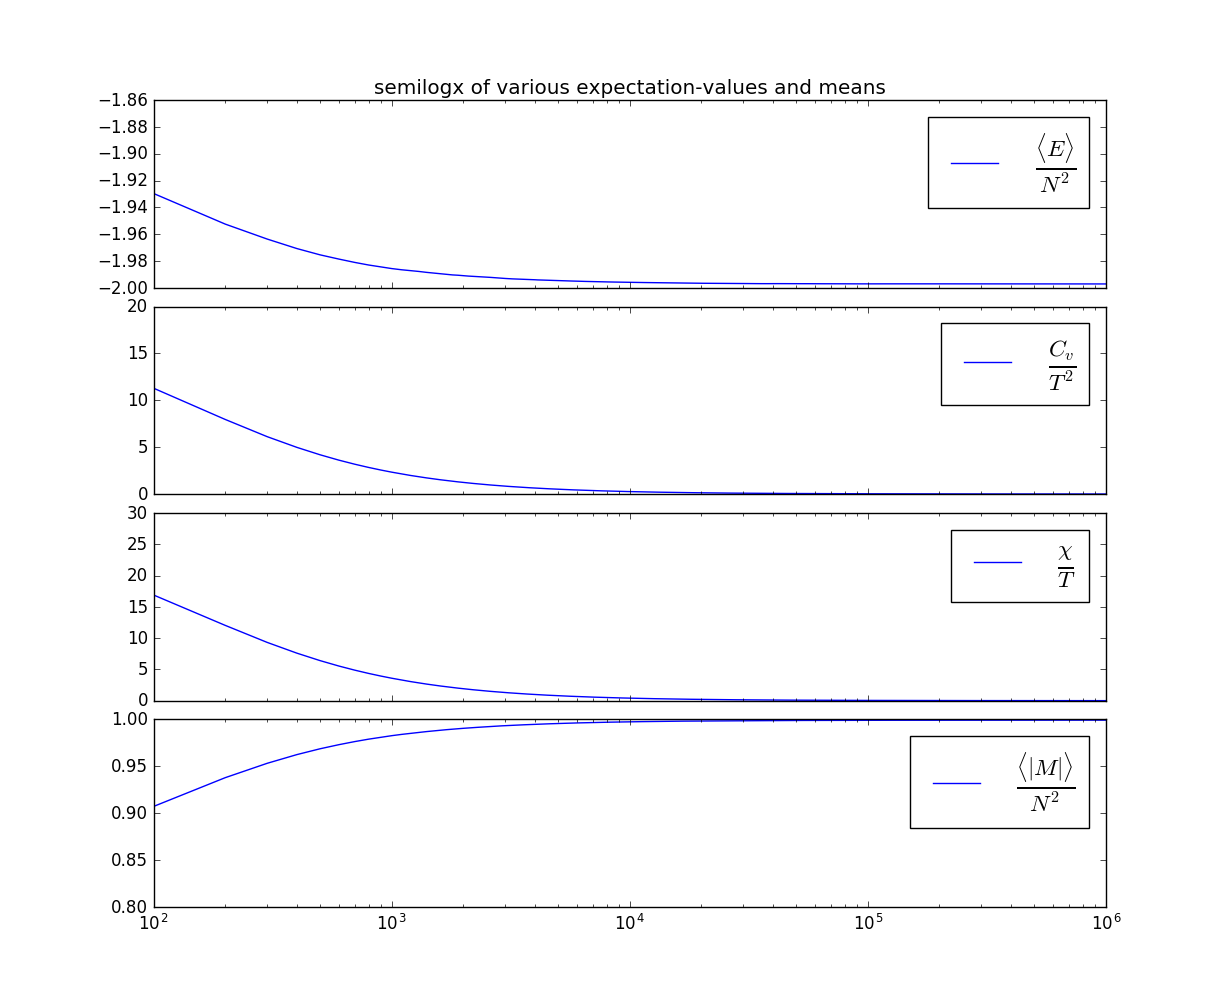
\includegraphics[scale=0.5]{exp_vals.png}\label{fig:exp_t1}
\caption{A set of plots for a temperature $T = 1.0$ and an initial configuration with spins in arbitrary up and down configurations with a lattice size $L = 20$. The x-axis denotes the number of monte carlo cycles and represents the time evolution of the system}
\end{figure}

\begin{figure}
\hspace*{-4cm}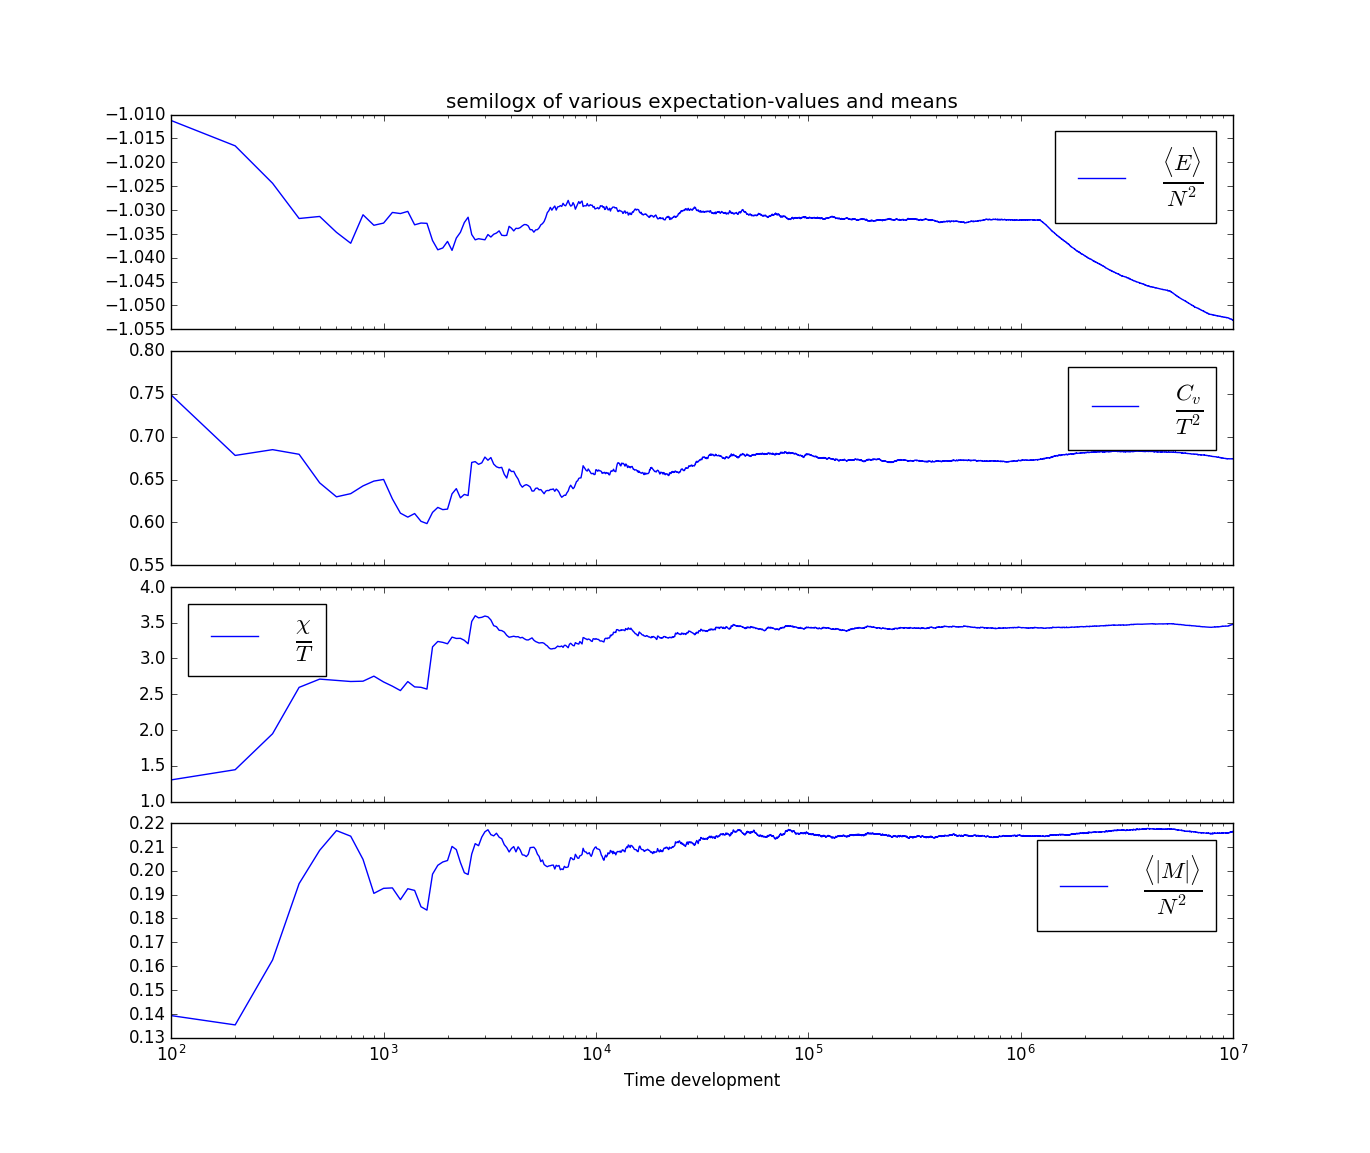
\includegraphics[scale=0.5]{exp_vals_2.png}\label{fig:exp_t2}
\caption{A set of plots for a temperature $T = 2.4$ and an initial configuration with spins in arbitrary up and down configurations with a lattice size $L = 20$. The x-axis denotes the number of monte carlo cycles and represents the time evolution of the system}
\end{figure}




\begin{figure}[H]
\hspace*{-1cm}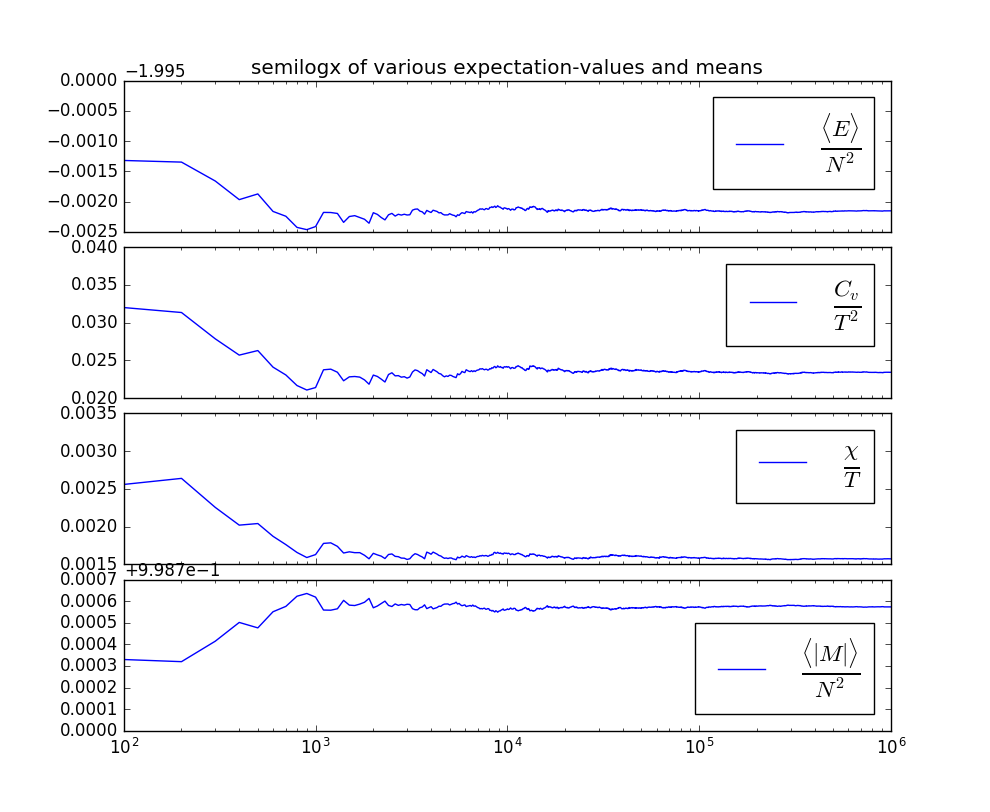
\includegraphics[scale=0.6]{exp_vals_ord_1.png}\label{fig:exp_t1_ord}
\caption{A set of plots for a temperature $T = 1.0$ and an initial configuration with spins all pointing the same direction and a lattice size of $L = 20 $. The x-axis denotes the number of monte carlo cycles and represents the time evolution of the system}
\end{figure}

\begin{figure}[H]
\hspace*{-1cm}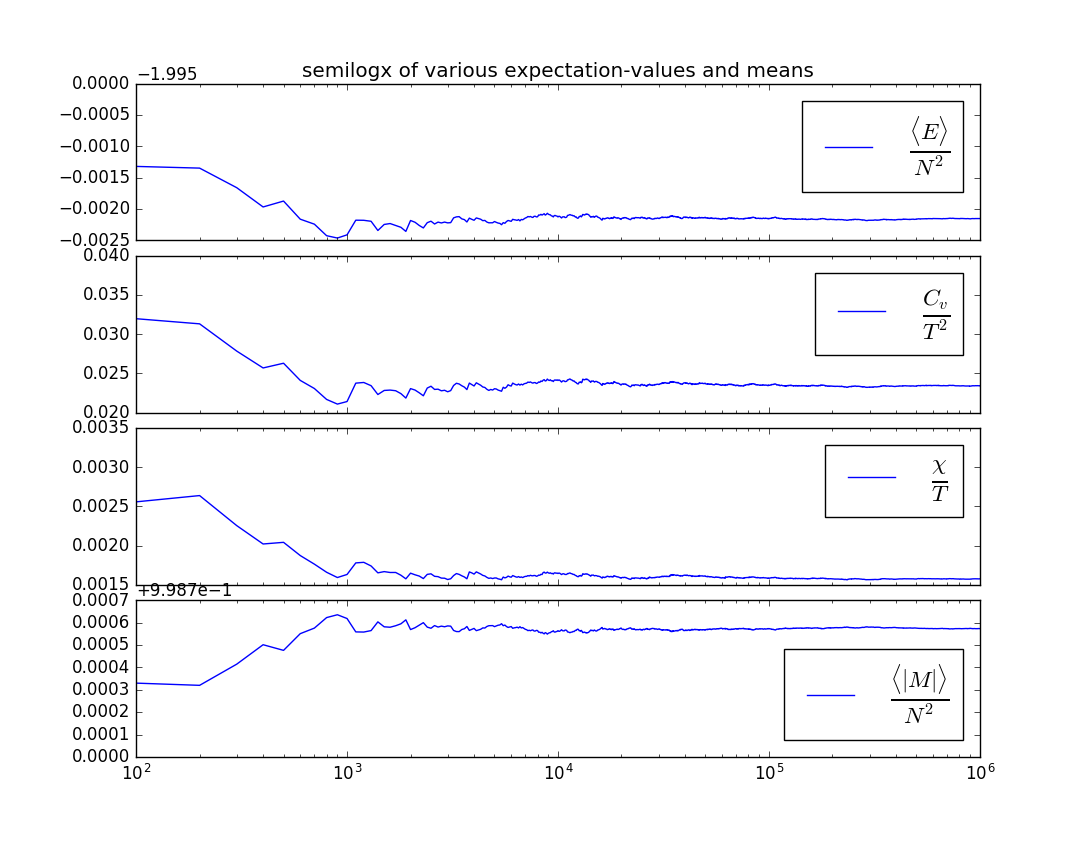
\includegraphics[scale=0.55]{exp_vals_ord_2.png}\label{fig:exp_t2_ord}
\caption{A set of plots for a temperature $T = 2.4$ and an initial configuration with spins all pointing the same direction and a lattice size of $L = 20 $. The x-axis denotes the number of monte carlo cycles and represents the time evolution of the system}
\end{figure}


\begin{figure}[H]
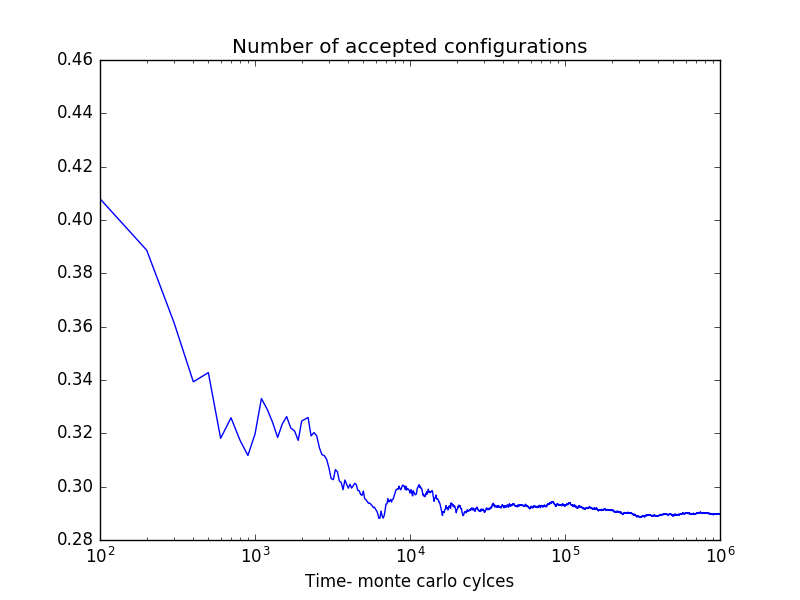
\includegraphics[scale=0.6]{accept_config_ord_1.png}\label{fig:accept_config_1_ord}
\caption{Presenting the number of accepted configurations according to the Metropolis test per number of monte - carlo cycles noted on the x-axis. This plot holds for a system with temperature $T = 1.0$, an initial configuration with spins all pointing the same direction and a lattice size of $L = 20 $}
\end{figure}

\begin{figure}[H]
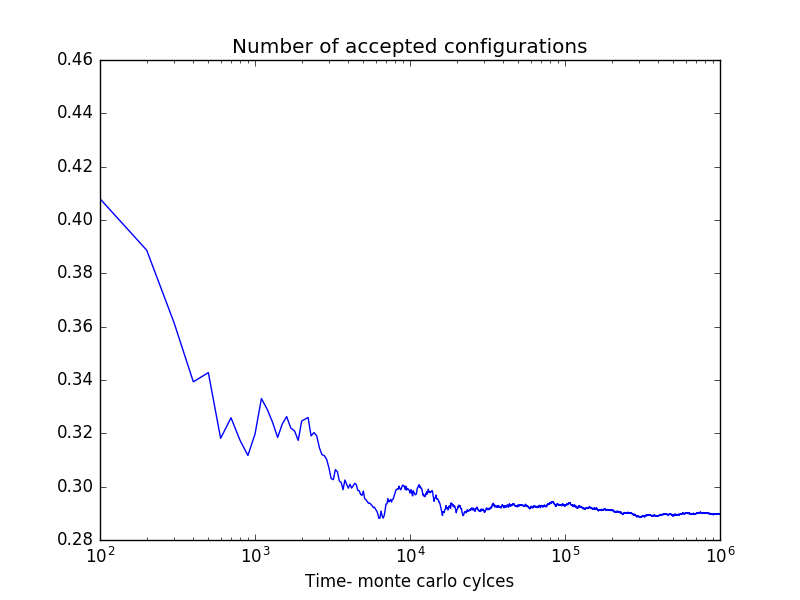
\includegraphics[scale=0.6]{accept_config_ord_2.png}\label{fig:accept_config_ord}
\caption{Presenting the number of accepted configurations according to the Metropolis test per number of monte - carlo cycles noted on the x-axis. This plot holds for a system with temperature $T = 2.4$, an initial configuration with spins all pointing the same direction, and a lattice size of $L = 20 $}
\end{figure}

\noindent 
\begin{figure}[H]
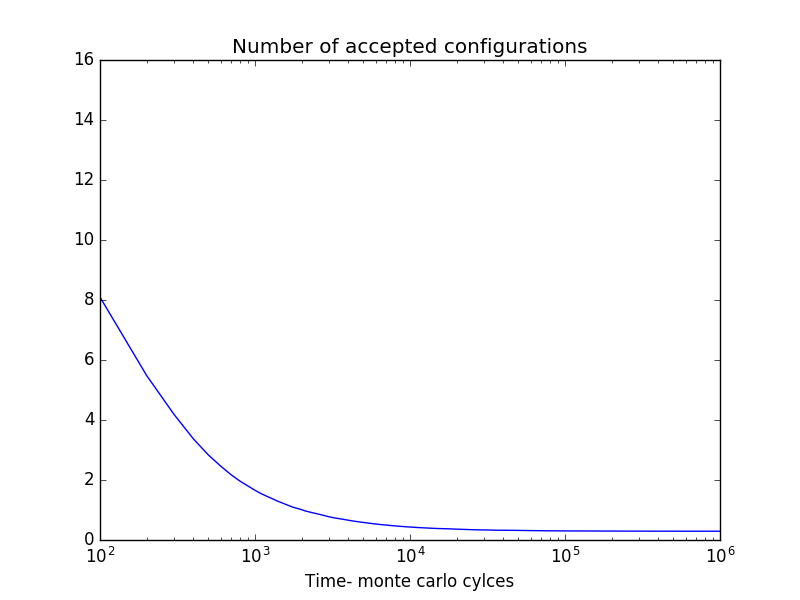
\includegraphics[scale=0.6]{accept_config_1.png}\label{fig:accept_config_1}
\caption{Presenting the number of accepted configurations according to the Metropolis test per number of monte - carlo cycles noted on the x-axis. This plot holds for a system with temperature $T = 1.0$, a configuration with spins in arbitrary states, and a lattice size of $L = 20 $}
\end{figure}

\begin{figure}[H]
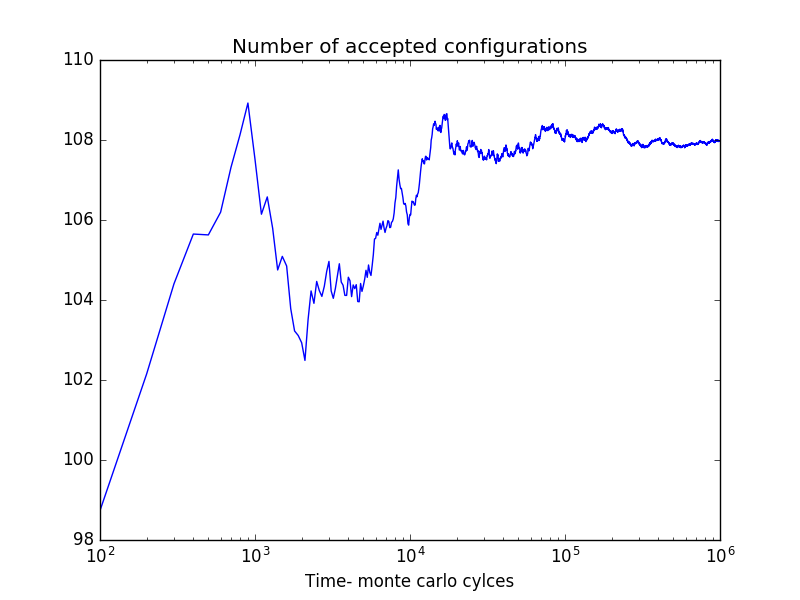
\includegraphics[scale=0.6]{accept_config.png}\label{fig:accept_config}
\caption{Presenting the number of accepted configurations according to the Metropolis test per number of monte - carlo cycles noted on the x-axis. This plot holds for a system with temperature $T = 2.4$, a configuration with spins in arbitrary states, and a lattice size of $L = 20 $}
\end{figure}



\section*{Discussion}

\subsection{4c}
Considereing the results presented in the figures \ref{fig:exp_t1} through \ref{fig:exp_t2_ord} there is a strong indication the  equilibrium time occurs in the area around $10^6$ cycles. Considering the behaviour of accepted configurations per cycle as a function of temperature in the system a systematic difference is found between the given temperatures. As shown in the difference between the figures \ref{fig:accept_config_1_ord} and \ref{fig:accept_config_ord} the number of accepted configurations per cycle is decreased significantly with temperature. This may be caused by an energy surplus in the  system causing more volatility (REF TO  EQUATION) (larger specter of energy values?)  
\section*{Conclusion}
\end{document}